
%\newcommand\map[5]{#1:#2\to#3,#4\mapsto#5}


\newcommand\map[3]{#1 : {#2}⟶  {#3}}
\newcommand\maps[5]{{#1}:{#2}⟶  {#3}, {#4} ↦ {#5}}

\aaa{Linear Transformations}%\a\aa\a\aa

Now Shinchan would start of making drinks, again he has the following recipe
\vfill
\[columns]{\co5
\t{}\cola\tea,\leaf11,\bean21.
\co5
\cola uses \fbox{\leaf\bean\bean}~\\
\vspace{2cm}
\tea uses \fbox{\leaf\bean}~\\
}

\a\aa
This time he would like to use pictures to organize those data. He \x{put} each product to the corresponding point in the linear combination space of materials.

\[columns]{\co7
\[z]{
\org
%\xaxis{-1}5
%\yaxis{-1}5
\grid{-3}{-3}33
%\wangge
\draw (1,0) node {\leaf} (0,1) node {\bean};
\draw (1,2) node {\cola} (1,1) node {\tea};
%\nnw A12
%\nnw B11
	}
\co3
\t{}\cola\tea,\leaf11,\bean21.
}

\a\aa
Onece again, he wants to combine two tables.

$$\t{}\cola\tea,\leaf11,\bean21.\quad\t{}\bento,\cola1,\tea1.=\t{}\bento,\leaf{},\bean{}.$$

You know how to do it. But how can he do it by \x{purly with pictures}?

\[columns]{\co5

\[zz]{
\org
\grid{-3}{-3}33
\draw (1,0) node {\sleaf} (0,1) node {\sbean};
\draw (1,2) node {\scola} (1,1) node {\stea};
	}
\co5
\[zz]{
\org
\grid{-3}{-3}33
\draw (1,0) node {\scola} (0,1) node {\stea};
\draw (1,1) node {\sbento};
	
}
}


\a\aa
He is confusing...... How to do it..... How to do it.... \x{Without computation}... How can he found the position of \sbento in the left picture.... How he can do matrix multiplication \x{purely geometrically}.....
\vfill
\[columns]{\co4

\[zz]{
\org
\grid{-2}{-2}22
\draw (1,0) node {\sleaf} (0,1) node {\sbean};
\draw (1,2) node {\scola} (1,1) node {\stea};
	}

Left Picture
\co4
\[zz]{
\org
\grid{-2}{-2}22
\draw (1,0) node {\scola} (0,1) node {\stea};
\draw (1,1) node {\sbento};
	
}

Right Picture
\co 2
\t{}\bento,\leaf{},\bean{}.
}


\a\aa
His chef come to his room and accidentally bumped on his picture.... 

Chef: Oh! I am sorry, Shinchan what are you doing here?


\[columns]{\co2

\[zz]{
\org
\grid{-2}{-2}22
\draw (1,0) node {\sleaf} (0,1) node {\sbean};
\draw (1,2) node {\scola} (1,1) node {\stea};
	}
Left Picture
\co3
\[zz]{
	\pgftransformcm{1}{2}{1}{1}{\pgfpoint{0}{0}}
\org
\grid{-1}{-1}11
\draw (1,0) node {\scola} (0,1) node {\stea};
\draw (1,1) node {\sbento};
	
}
Right Picture
\co 2
\t{}\bento,\leaf{},\bean{}.
}

Shinchan: Oh!!! No!!! My pictures, you destroyed my picture...

\a\aa
Chef: I am sorry, but... Are there any difference with those two pictures?
\vfill
\[columns]{\co3

\[zzz]{
\org
\grid{-1}{-1}11
\draw (1,0) node {\scola} (0,1) node {\stea};
\draw (1,1) node {\sbento};
}

Right Picture BEFORE
\co 3

$\leftarrow$ Any difference? $\rightarrow$
\co4
\[zzz]{[x={(1,1)},y={(2,1)}]
\pgftransformcm{2}{0.8}{1.4}{2}{\pgfpoint{5cm}{5cm}}
\org
\grid{-1}{-1}11
\draw (1,0) node {\scola} (0,1) node {\stea};
\draw (1,1) node {\sbento};
}
Right Picture AFTER



}
\a\aa

After the Chef explained, Shinchan knows this crooked picture \x{keeps all information of the recipe table} because it \x{keeps} the \x{parallelgrams}, the vector for tea \stea and for cola \scola, still adds to the vector for \sbento.

\[columns]{\co 7

\[zzz]{[x={(1,1)},y={(2,1)}]
\pgftransformcm{2}{0.8}{1.4}{2}{\pgfpoint{5cm}{5cm}}
\org
\grid{-2}{-2}22
\draw (1,0) node {\scola} (0,1) node {\stea};
\draw (1,1) node {\sbento};
\draw[->,thick,red] (0,0)--(1,0);
\draw[ultra thick,dotted,red] (0,1)--(1,1);
\draw[->,thick,green!80!black] (0,0)--(0,1);
\draw[ultra thick,dotted,green!80!black] (1,0)--(1,1);
}
\co 3
\t{}\bento,\cola1,\tea1.
}


\a\aa

Shinchan: Great! I am trying to compute matrix multiplication geometrically. I have a recipe to make \x{intermidiates} from \x{materials}, and to make \x{final meals} from \x{intermidiates}. I wish to figure out how to make \x{final meals} from \x{materials}. What should I do?




\[columns]{\co2

\[zz]{
\org
\grid{-2}{-2}22
\draw (1,0) node {\sleaf} (0,1) node {\sbean};
\draw (1,2) node {\scola} (1,1) node {\stea};
	}
Left Picture
\co3
\[zz]{
	\pgftransformcm{1}{2}{1}{1}{\pgfpoint{0}{0}}
\org
\grid{-1}{-1}11
\draw (1,0) node {\scola} (0,1) node {\stea};
\draw (1,1) node {\sbento};
	
}
Right Picture
\co 2
\t{}\bento,\leaf{},\bean{}.
}





\a\aa


\[columns]{\co7
\[z]{
\org
\grid{-3}{-3}33
\draw[color=blue] (1,0) circle[radius=0.3] node {\sleaf} (0,1) circle[radius=0.3] node {\sbean};
\draw[color=red] (1,2) circle[radius=0.3] node {\scola} (1,1) circle[radius=0.3] node {\stea};
	}

\co3
Chef: Now I see you have the Left Picture. That represents how you make {\color{red} drinks} out of {\color{blue}materials}

\vspace{.3cm}
\vfill


\t{}\cola\tea,\leaf11,\bean21.


}


\a\aa


\[columns]{\co7
\[z]{
\org
	\pgftransformcm{1}{2}{1}{1}{\pgfpoint{0}{0}}
\grid[red!60!white!40]{-1}{-1}11
\draw[color=orange] (1,1) circle[radius=0.3] node {\sbento};
\draw[color=red] (0,1) circle[radius=0.3] node {\scola};
\draw[color=red] (1,0) circle[radius=0.3] node {\stea};
	}

\co3


Chef: And I see you have the Right Picture, which represents how to make {\color{orange}meal}s out of {\color{red}drinks}. Oh I am sorry to bump it...Hopefully we do not lose any information.
\vfill
\vspace{.3cm}
\quad\t{}\bento,\cola1,\tea1.
}



\a\aa









\[columns]{\co7
\[z]{
\org
\grid{-3}{-3}33
\draw[color=blue] (1,0) circle[radius=0.3] node {\sleaf} (0,1) circle[radius=0.3] node {\sbean};
\draw[color=red] (1,2) circle[radius=0.3] node {\scola} (1,1) circle[radius=0.3] node {\stea};
\draw[color=orange] (2,3) circle[radius=0.3] node {\sbento};
	\pgftransformcm{1}{2}{1}{1}{\pgfpoint{0}{0}}
\grid[red!60!white!40]{-1}{-1}11
%\draw (1,1) node {\sbento};
	}

\co3
Oh! Let us simply put those two picture together!! Then it shows up all information. We now know how to make {\color{orange}meals} \sbento by {\color{blue}materials} \sleaf, \sbean. 
\vspace{.3cm}

\t{}\bento,\leaf2,\bean3.
}



















\a\aa

Let's summarise the \x{Geometric method} of computing matrix multiplication.

\textbf{Step 1:} We have two pictures corresponding to the left factor and the right factor.



\[columns]{
\co 5

\[zzz]{
\org
\grid{-2}{-2}22
\draw[color=blue] (1,0) circle[radius=0.3] node {\sleaf} (0,1) circle[radius=0.3] node {\sbean};
\draw[color=red] (1,2) circle[radius=0.3] node {\scola} (1,1) circle[radius=0.3] node {\stea};
}

Left factor: Making {\color{red} drinks} by {\color{blue}materials}

\t{}\cola\tea,\bean21,\leaf11.
\co 5

\[zzz]{
\org
%	\pgftransformcm{1}{2}{1}{1}{\pgfpoint{0}{0}}
\grid[red!60!white!40]{-1}{-1}11
\draw[color=orange] (1,1) circle[radius=0.3] node {\sbento};
\draw[color=red] (0,1) circle[radius=0.3] node {\scola};
\draw[color=red] (1,0) circle[radius=0.3] node {\stea};
	}

Right factor: Making {\color{orange} meals} by {\color{red}drinks}

\t{}\bento,\tea1,\cola1.
}





\a\aa

\textbf{Step 2:} Skew the right picture so that the relative position of {\color{red} drinks} matches its position in the left picture.



\[columns]{
\co 5

\[zzz]{
\org
\grid{-2}{-2}22
\draw[dotted, color=red] (0,0)--(1,1) (0,0)--(1,2);
\draw[color=blue] (1,0) circle[radius=0.3] node {\sleaf} (0,1) circle[radius=0.3] node {\sbean};
\draw[color=red] (1,2) circle[radius=0.3] node {\scola} (1,1) circle[radius=0.3] node {\stea};
}

Left factor: Making {\color{red} drinks} by {\color{blue}materials}

%\t{}\cola\tea,\bean21,\leaf11.
\co 5

\[zzz]{
\org
	\pgftransformcm{1}{2}{1}{1}{\pgfpoint{0}{0}}
\grid[red!60!white!40]{-1}{-1}11
\draw[color=orange] (1,1) circle[radius=0.3] node {\sbento};
\draw[color=red] (0,1) circle[radius=0.3] node {\scola};
\draw[color=red] (1,0) circle[radius=0.3] node {\stea};
	}

Right factor: Making {\color{orange} meals} by {\color{red}drinks}

%\t{}\bento,\tea1,\cola1.
}


\a\aa


\textbf{Step 3:} Put them together, then you can see how to make a {\color{orange}meal} \bento by {\color{blue}materials} \leaf,\bean. You got the matrix multiplication.





\[z]{
\org
\grid{-3}{-3}33
\draw[color=blue] (1,0) circle[radius=0.3] node {\sleaf} (0,1) circle[radius=0.3] node {\sbean};
\draw[color=red] (1,2) circle[radius=0.3] node {\scola} (1,1) circle[radius=0.3] node {\stea};
\draw[color=orange] (2,3) circle[radius=0.3] node {\sbento};
	\pgftransformcm{1}{2}{1}{1}{\pgfpoint{0}{0}}
\grid[red!60!white!40]{-1}{-1}11
%\draw (1,1) node {\sbento};
	}





\a\aa

The whole process is a \x{map}. The domain of the map is the linear combination space of {\color{red} drinks}. The codomain(target) of the map is the linear combination space of {\color{blue} materials}. The process skews the picture of the domain and put it to the codomain.  

\[columns]{
\co4

\[zz]{
\org
%	\pgftransformcm{1}{2}{1}{1}{\pgfpoint{0}{0}}
\grid[red!60!white!40]{-1}{-1}11
\draw[color=orange] (1,1) circle[radius=0.3] node {\sbento};
\draw[color=red] (0,1) circle[radius=0.3] node {\scola};
\draw[color=red] (1,0) circle[radius=0.3] node {\stea};
	}

Domain: space of {\color{red} drinks}. Corresponds to \x{right factor}.
\co1
$$\longrightarrow$$
\co5

\[zzz]{
\org
\grid{-3}{-3}33
\draw[color=blue] (1,0) circle[radius=0.3] node {\sleaf} (0,1) circle[radius=0.3] node {\sbean};
\draw[color=red] (1,2) circle[radius=0.3] node {\scola} (1,1) circle[radius=0.3] node {\stea};
\draw[color=orange] (2,3) circle[radius=0.3] node {\sbento};
	\pgftransformcm{1}{2}{1}{1}{\pgfpoint{0}{0}}
\grid[red!60!white!40]{-1}{-1}11
%\draw (1,1) node {\sbento};
	}

Codomain: space of {\color{blue} materials}. Corresponds to \x{left factor}.

}



\a\aa




\[columns]{
\co4

\[zz]{
\org
%	\pgftransformcm{1}{2}{1}{1}{\pgfpoint{0}{0}}
\grid[red!60!white!40]{-1}{-1}11
\draw[color=orange] (1,1) circle[radius=0.3] node {\sbento};
\draw[color=red] (0,1) circle[radius=0.3] node {\scola};
\draw[color=red] (1,0) circle[radius=0.3] node {\stea};
	}

\co1
$$\longrightarrow$$
\co5

\[zzz]{
\org
\grid{-3}{-3}33
\draw[color=blue] (1,0) circle[radius=0.3] node {\sleaf} (0,1) circle[radius=0.3] node {\sbean};
\draw[color=red] (1,2) circle[radius=0.3] node {\scola} (1,1) circle[radius=0.3] node {\stea};
\draw[color=orange] (2,3) circle[radius=0.3] node {\sbento};
	\pgftransformcm{1}{2}{1}{1}{\pgfpoint{0}{0}}
\grid[red!60!white!40]{-1}{-1}11
%\draw (1,1) node {\sbento};
	}


}



The only restriction for this map is that: The whole process maps parallelograms to parallelograms and it maps origin to origin. In Math, this is called a \x{Linear Transformation}. 




\a\aa
\[defi]{
A linear transformation is a map $\map TVW$ for linear spaces $V,W$ over $F$ such that
$$
T(\vv+\ww)=T(\vv)+T(\ww)\qquad T(\lambda\vv)=\lambda T(\vv)
$$ 
for any $\vv,\ww\in V$ and $\lambda\in F$.

We call $V$ the \x{Domain} of $T$, $W$ the \x{Codomain} of $T$.
}
\[defi]{
The linear transformation $\map TVV$ in the case domain equals the codomain is called a \x{Linear Operator}.
}
\a\aa
$$
T(\vv+\ww)=T(\vv)+T(\ww)\qquad T(\lambda\vv)=\lambda T(\vv)
$$ is a condition of saying keeping parallelograms.
%\vfill
%Those parallelgrams, includes collapsed parallelograms, that is a point or a line segment.
\vfill
As we have shown here, linear transformation gives a \x{geometric understanding} of matrix multiplication. 

\a\aa
\[prop]{If $\map TVW$ is a linear transformation, then for any $\vv_1,\cdots\vv_n\in V$, $a_1,\cdots,a_n\in\RR$, we have
$$
T(a_1\vv_1+\cdots+a_n\vv_n)=a_1T(\vv_1)+\cdots+a_nT(\vv_n).
$$
}
In other words, linear transformation preserves the coefficient of linear combination. 
\vfill

\[proof]{
	\[equation*]{\[split]{
		T(a_1\vv_1+\cdots+a_n\vv_n)&=T((a_1\vv_1+\cdots+a_{n-1}\vv_{n-1})+a_n\vv_n)\\
		&=T(a_1\vv_1+\cdots+a_{n-1}\vv_{n-1})+a_nT(\vv_n)
		}}
Then using induction	
	}

\a\aa





There are other geometric examples of linear transoformations.




\begin{tikzpicture}[scale=0.5]
\draw[thick] (0cm,0cm) circle(1cm);
\draw[thick] plot [smooth,tension=1.5] coordinates{(-0.5,-0.5) (0,-0.8) (0.5,-0.5)};
\draw [thick, fill=black] (0,-0.2) circle (0.1);
\draw[thick] plot [smooth,tension=1.5] coordinates{(-0.4,0.4) (-0.3,0.5) (-0.2,0.4)};
\draw[thick] plot [smooth,tension=1.5] coordinates{(0.4,0.4) (0.3,0.5) (0.2,0.4)};
\draw[thick] (8cm,0cm) circle(1cm);
\draw[thick] plot [smooth,tension=1.5] coordinates{(7.5,0.5) (7.2,0) (7.5,-0.5)};
\draw [thick, fill=black] (7.8,0) circle (0.1);
\draw[thick] plot [smooth,tension=1.5] coordinates{(8.4,0.4) (8.5,0.3) (8.4,0.2)};
\draw[thick] plot [smooth,tension=1.5] coordinates{(8.4,-0.4) (8.5,-0.3) (8.4,-0.2)};
\draw[thick,->,orange](2.8,0.1)--(6.8,0.1) node[near start, above]{};
%\draw[thick,->,orange](5.8,-0.6)--(1.8,-0.6) node[near start, below]{Rotation by 90 degree counterclockwise};
\end{tikzpicture}Rotation by 90 degree.

\vspace{0.3cm}


\begin{tikzpicture}[scale=0.5]
\draw[thick] (0cm,0cm) circle(1cm);
\draw[thick] plot [smooth,tension=1.5] coordinates{(-0.5,-0.5) (0,-0.8) (0.5,-0.5)};
\draw [thick, fill=black] (0,-0.2) circle (0.1);
\draw[thick] plot [smooth,tension=1.5] coordinates{(-0.4,0.4) (-0.3,0.5) (-0.2,0.4)};
\draw[thick] plot [smooth,tension=1.5] coordinates{(0.4,0.4) (0.3,0.5) (0.2,0.4)};
\draw[thick] (8cm,0cm) circle(1cm);
\draw[thick] plot [smooth,tension=1.5] coordinates{(7.5,0.5) (8,0.8) (8.5,0.5)};
\draw [thick, fill=black] (8,0.2) circle (0.1);
\draw[thick] plot [smooth,tension=1.5] coordinates{(7.6,-0.4) (7.7,-0.5) (7.8,-0.4)};
\draw[thick] plot [smooth,tension=1.5] coordinates{(8.4,-0.4) (8.3,-0.5) (8.2,-0.4)};
\draw[thick,->,orange](2.8,0.1)--(6.8,0.1) node[near start, above]{};
%\draw[thick,->,orange](5.8,-0.6)--(1.8,-0.6) node[near start, below]{Rotation by 90 degree counterclockwise};
\end{tikzpicture}Reflection horizontally

\vspace{0.3cm}

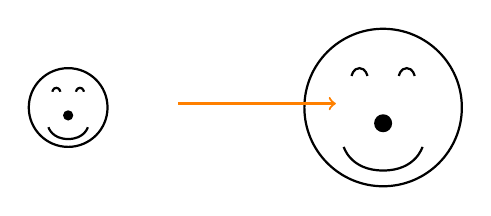
\begin{tikzpicture}[scale=0.5]
\draw[thick] (0cm,0cm) circle(1cm);
\draw[thick] plot [smooth,tension=1.5] coordinates{(-0.5,-0.5) (0,-0.8) (0.5,-0.5)};
\draw [thick, fill=black] (0,-0.2) circle (0.1);
\draw[thick] plot [smooth,tension=1.5] coordinates{(-0.4,0.4) (-0.3,0.5) (-0.2,0.4)};
\draw[thick] plot [smooth,tension=1.5] coordinates{(0.4,0.4) (0.3,0.5) (0.2,0.4)};
\draw[thick] (8cm,0cm) circle(2cm);
\draw[thick] plot [smooth,tension=1.5] coordinates{(7,-1) (8,-1.6) (9,-1)};
\draw [thick, fill=black] (8,-0.4) circle (0.2);
\draw[thick] plot [smooth,tension=1.5] coordinates{(7.2,0.8) (7.4,1) (7.6,0.8)};
\draw[thick] plot [smooth,tension=1.5] coordinates{(8.8,0.8) (8.6,1) (8.4,0.8)};
\draw[thick,->,orange](2.8,0.1)--(6.8,0.1) node[near start, above]{};
%\draw[thick,->,orange](5.8,-0.6)--(1.8,-0.6) node[near start, below]{Rotation by 90 degree counterclockwise};
\end{tikzpicture}Scalling

\vspace{0.3cm}

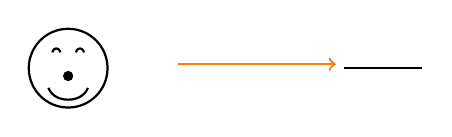
\begin{tikzpicture}[scale=0.5]
\draw[thick] (0cm,0cm) circle(1cm);
\draw[thick] plot [smooth,tension=1.5] coordinates{(-0.5,-0.5) (0,-0.8) (0.5,-0.5)};
\draw [thick, fill=black] (0,-0.2) circle (0.1);
\draw[thick] plot [smooth,tension=1.5] coordinates{(-0.4,0.4) (-0.3,0.5) (-0.2,0.4)};
\draw[thick] plot [smooth,tension=1.5] coordinates{(0.4,0.4) (0.3,0.5) (0.2,0.4)};
\draw[thick] (7,0)--(9,0);
\draw[thick,->,orange](2.8,0.1)--(6.8,0.1) node[near start, above]{};
%\draw[thick,->,orange](5.8,-0.6)--(1.8,-0.6) node[near start, below]{Rotation by 90 degree counterclockwise};
\end{tikzpicture}Projecting




















\a\aa
In space of functions, linear transformations happens when we \x{change varibles} or make \x{linear combination of functions}. For example, let $P_\infty$ be the space of all polynomials. The map defined by 
$$\maps{T}{P_\infty}{P_\infty}{f(x)}{f(x^2)}$$ is \x{linear}, (\exe: Check it). 
\vfill
Remember to check that the expression $f(x^2)$ you defined is \x{actually} an element in the codomain. For example, if $P_2$ is the sapce of all polynomials of degree at most 2. The following argument
$$
\maps T{P_2}{P_2}{f(x)}{f(x^2)}
$$
\x{is not even a map} ($x^2\mapsto x^4\notin P_2$)

\a\aa
You can also define linear transformation on set of functions by \x{linearly combine its function values}, \x{derivative}, or \x{integration} for example
$$
T:f(x)\mapsto f(1+\sqrt{x})+f(1-\sqrt{x});\qquad T:f(x)\mapsto xf(x)+x^2f(x)\quad $$$$T:f(x)\mapsto f'(x);\qquad T:f(x)\mapsto \int_0^x f(t)\dd t.
$$
\vfill
%The map $f\mapsto f'$ can be thought like linear combination of $f(x)$ with $f(x+0.01)$ with coefficient $-100f(x)+100f(x+0.01)$, but here in case of $f'$ the number $0.01$ and $100$ can be thought as replaced by infinitesimal and infinite numbers.

\a{Linear space of linear transformation}
Let $S$ be a set, $V$ a linear space, consider the set of all \x{maps}
$$
\Hom_{\mathrm{set}}(S,V):=\left\{f|\map fSV\right\}
$$
\vfill
This set is \x{a linear space }under the following addition and scalar multiplication
\vfill
For any $f,g\in \Hom_{\mathrm{set}}(S,V)$ and $\lambda,\mu\in F$, $s\in S$
$$
(\lambda f+\mu g)(s):=\lambda f(s)+\mu g(s).
$$
\vfill
\exe : Verify $\Hom_{\mathrm{set}}(S,V)$ is a linear space.
\a\aa
\exe Let $V,W$ be linear spaces over $F$, use the following symbol to denote the set all linear transformations from $W$ to $V$
$$
\mathcal L(W,V):=\left\{f|\map fWV \text{ linear transformation }\right\}
$$
We define addition and scalar multiplication for any $f,g\in \mathcal L(W,V)$ and $\lambda,\mu\in F$, $\ww\in W$ by

$$
(\lambda f+\mu g)(s):=\lambda f(s)+\mu g(s).
$$

Verify $\mathcal L(W,V)$ is a linear space.

\vspace{3cm}

\a{Verify a map is a linear transformation}
To verify a map $\map TVW$ is a linear tranformation, we only need
\vfill
\[itemize]{
\item Write down expression of $\vv_1,\vv_2$ for arbitrary element $\vv\in V$. 
\item Check the element is well-defined and it defined to be an element in codomain.
\item Compute $T(\lambda\vv_1+\vv_2)$ for arbitrary element $\lambda\in F$
\item Compare with $\lambda T(\vv_1)+T(\vv_2)$.
	}
We only verify $T(\lambda\vv_1+\vv_2)$ is because the following
\[prop]{For any map $T$, if $T(\lambda\vv_1+\vv_2)=\lambda T(\vv_1)+T(\vv_2)$, this is a linear tranformation.}
\[proof]{$T(\lambda\vv_1+\mu\vv_2)=\lambda T(\vv_1)+ T(\mu\vv_2)=\lambda T(\vv_1)+ \mu T(\vv_2)$}
\a\aa
\exe Let $P_2$ be the space of polynomials of degree at most 2. Show that the following map
$$
\maps T{P_2}{P_2}{f(x)}{f(1+\sqrt x)+f(1-\sqrt x)}
$$
is a linear transformation.

\sol Let $f,g$ be arbitrary polynomials in $P_2$, so there exists unique $a,b,c,d,e,f\in F$ so $f,g$ can be written as\footnote{The use of \pa $a,b,c,d,e,f$  is an example of \enu}
\[equation]{\label{para}
f(x)=ax^2+bx+c\qquad g(x)=dx^2+ex+f.
}
We first show that $T[f]\in P_2$. Indeed,
$$
T[f](x)=f(1+\sqrt x)+f(1-\sqrt x)
$$

\a\aa

Plug \eqref{para} in, we have

$$
T[f](x)=a(1+\sqrt x)^2+b(1+\sqrt x)+c + a(1-\sqrt x)^2+b(1-\sqrt x)+c
$$

By computation, this expression equals to $$a(2+x^2)+2b+2c\in P_2.$$

To check linear, note that for any scalar $\lambda\in f$
$$
T[\lambda f+g]=\lambda f(1+\sqrt x)+\lambda f(1-\sqrt x)+g(1+\sqrt x)+g(1-\sqrt x)=\lambda T[f]+T[g]
$$
So $T$ is a linear tranformation.

\a\aa
\exe Choose an element $s\in S$. Let $V$ be a linear space, $\Hom_{\mathrm{set}}(S,V)$ is the set of maps with domain $S$ and codomain $V$. Previously we proved it is a linear space. Consider the \x{map of evaluation at $s$ } 
$$
\maps{E_s}{\Hom_{\mathrm{set}}(S,V)}Vf{f(s)}
$$

Prove that this is a linear transformation. 

\vspace{3cm}



\a{Non-linear transformations}
Non-linear transformations always happens when we combine values of functions in a non-linear way, like $f(x)\mapsto f(x)^2$ or $f(x)\mapsto \sqrt{f(x)}$. To disprove linearity, we only need to choose some coefficient such that the definition of linear transformation not work.
\vfill
Sometimes, we write $T[f]$ to denote the output function when apply linear transfomation of $T$.

\a\aa
\exe Let $V$ be the space of all polynomials over $\RR$. Show that $T[f](x)=f(x)^2$ is not a linear transformation.
\vfill
\sol: Let $$\[cases]{f_1(x)=1\\f_2(x)=x}$$, then $$T[f_1+f_2](x)=(1+x)^2=1+x^2+2x$$
But
$$T[f_1](x)+T[f_2](x)=1+x^2.$$
So 
$$
T[f_1+f_2]\neq T[f_1]+T[f_2]
$$
This is not a linear transformation.


\aaa
